% Preamble {{{
\documentclass[12pt]{report} %N
\usepackage[margin=1in]{geometry}
\geometry{
left=1.2in
}
\usepackage[
backend=biber,
style=numeric,
sorting=none
]{biblatex}
\addbibresource{citations.bib}
\usepackage{graphicx}
\usepackage{float}
\usepackage{array}
\usepackage{caption}
\usepackage{amsmath}
\usepackage{ragged2e}
\usepackage{listings}
\usepackage{titlesec}
\usepackage{hyperref}
\usepackage{longtable}
\hypersetup{
    colorlinks=true,
		citecolor=black,
    linkcolor=black,
    filecolor=magenta,      
    urlcolor=cyan,
    pdfpagemode=FullScreen,
    }

\lstset{
basicstyle=\small\ttfamily,
columns=flexible,
breaklines=true
}

% Chapter title formatting
\titleformat{\chapter}[display]
  {\normalfont\huge\bfseries\centering}{\centering\chaptertitlename\ \thechapter}{20pt}{\Huge} 
\titlespacing*{\chapter} 
  {0pt}{50pt}{40pt}

% Recompile these documents. Do this if you're currently making changes to title and introcution chapters
% \includeonly{
	% chapters/title,
	% chapters/introduction,
% }
% }}}

\begin{document}

% Title page %N{{{
\thispagestyle{empty}
\begin{center}
\begin{minipage}{0.75\linewidth}
    \centering

%Thesis title
    {\uppercase{\Huge \textbf{PRAMANIT}
\par}}

\vspace{1cm}
{\LARGE \textbf{  Kedar Devasthali - 227668} \par }
{\LARGE \textbf{ Shivam Naik - 227681} \par}
{\LARGE \textbf{ Riddhi  Siddarkar - 227727} \par}
{\LARGE \textbf{ T.S. Vishwak - 227736} \par}
\vspace{1cm}
\end{minipage}
\end{center}

\noindent 	{Project Report
		Submitted in partial fulfillment of the requirements
		For the degree of\par}

		\begin{center}
			
			\vspace{1cm}
			{\Large \textbf{BACHELOR OF ENGINEERING}\par}
			{\Large \textbf{Branch: Computer Engineering}\par}
			\vspace{1cm}
			%Author's name
			
			
			%Guide
			{\Large \textbf {OF GOA UNIVERSITY}\par}
			
			\vspace{1.5cm}
			%University logo
			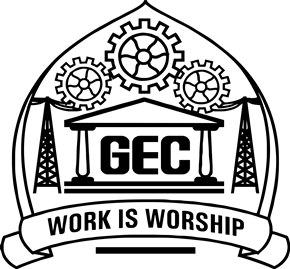
\includegraphics[width=0.2\linewidth]{gecLogo.png}
			\par
			
			%University Name
			\vspace{1.5cm}
			{\Large \textbf{AUGUST 2022}\par}
			\vspace{1.5cm}
			{\Large \textbf{COMPUTER ENGINEERING DEPARTMENT} \par}
			\vspace{0.3cm}
			{\LARGE \textbf{Goa College of Engineering} \par}
			{\textbf{(GOVERNMENT OF GOA)} \par}
			{\Large \textbf{FARMAGUDI, PONDA, GOA - 403401} \par}
		
		\end{center}
			\clearpage
			%}}}


% Title page %N{{{
    \thispagestyle{empty}
    \begin{center}
        {\Large \textbf{GOA COLLEGE OF ENGINEERING} \par}
        {\textbf{(GOVERNMENT OF GOA)} \par}
        {\Large \textbf{FARMAGUDI, PONDA, GOA - 403401} \par}
    \vspace{1cm}

    %Thesis title
    {\uppercase{\Huge \textbf {PRAMANIT}}
\par}
        \vspace{1cm} {\large { Bona fide record of work done by} \par }
    \vspace{1cm}
        {\Large{ \textbf{ Kedar Devasthali } 181105017}\par }
        {\Large \textbf{ Shivam Naik }181105036 \par}
        {\Large \textbf{ Riddhi  Siddarkar }181105058 \par}
        {\Large \textbf{ T.S. Vishwak }181105060 \par}
        \vspace{0.5cm}
        
    \end{center}
        {\noindent { Project Report submitted in partial fulfillment of the requirements for the degree of} \par }
        \begin{center}
            
        {\Large \textbf{BACHELOR OF ENGINEERING}\par}
        {\Large \textbf{Branch: Computer Engineering}\par}
        {\Large \textbf {OF GOA UNIVERSITY}\par}
        {\Large \textbf{AUGUST 2022}\par}
        \vspace{1.5cm}
        

    \end{center}
    \begin{table}[H]
        \begin{center}
    \begin{tabular}{lcl}
        \noindent ----------------------------------- &\hspace{1cm}&  ----------------------------------- \\
    Dr Gajanan Gawde & \hspace{3cm} & Dr. Jayapura A. Laxminarayana  \\
    Faculty guide        & \hspace{3cm} & Head of Computer Engg Dept    \\
    \end{tabular}
    \end{center}
\end{table}
\hrule
\vspace{.8cm}
{\noindent {Certified that the candidate was examined in the viva-voce examination held on ……} \par }
\vspace{1.5cm}
\begin{table}[H]
    \begin{center}
\begin{tabular}{lcl}
    \noindent ----------------------------------- &\hspace{1cm}&  ----------------------------------- \\
    (Internal Examiner) & \hspace{3cm} &   (External Examiner) \\
\end{tabular}
\end{center}
\end{table}
    \clearpage
    %}}}
%DO NOT MESS AROUND WITH THE CODE ON THIS PAGE UNLESS YOU %REALLY KNOW WHAT YOU ARE DOING
%E
\begin{center}
\underline{\bfseries \huge PROJECT APPROVAL SHEET}\\
\vspace{1cm}
\end{center}
\noindent This is to certify that \textbf{Shri Kedar Devasthali} (bearing Seat no. 228680), \textbf{Shrimati Riddhi Siddarkar} (bearing Seat no. 228725), \textbf{Shri Shivam Naik} (bearing Seat no. 228703) and \textbf{Shri T. S. Vishwak} (bearing Seat no. 228729) has been admitted to semester VII to the candidacy of degree (Bachelor of Engineering in Computer Engineering) in 2021-2022 and he/she has undertaken the dissertation entitled "\textbf{PRAMANIT: Decentralized Application to store and verify the authenticity of Birth and Death Certificates.}" which is approved for the degree of BE (Computer) under Goa University as it is found satisfactory

\vspace{2.8cm}

\begin{table}[H]
	\begin{center}
\begin{tabular}{lcl}
	\noindent ----------------------------------- &\hspace{1cm}&  ----------------------------------- \\
	(Internal Supervisor ) & \hspace{3cm} & (External Supervisor) \\
Dr Gajanan Gawde & \hspace{3cm}   \\
Associate Professor, Computer Dept. & \hspace{3cm}  \\
\end{tabular}
\end{center}
\end{table}

\vspace{2.5cm}

\begin{table}[H]
	\begin{center}
		\begin{tabular}{lcl}
			\noindent ----------------------------------- &\hspace{1cm}&  ----------------------------------- \\
		(Head of Department) & \hspace{3cm} & (Principal) \\
		Prof. Dr. J. A. Laxminarayanan & \hspace{3cm} &Dr. Rajesh Lohani \\
		Professor, Computer Dept. & \hspace{3cm} & Goa College of Engineering \\
		\end{tabular}
		\end{center}
\end{table}

\vspace{2cm}

\noindent Date: \\
\\
\noindent Place: \\

% \noindent Place: Farmagudi, Ponda, Goa\\
% \noindent Date: 



\tableofcontents

\addcontentsline{toc}{section}{Acknowlegdement}

\begin{center}
    \underline{\bfseries \huge ACKNOWLEDGEMENT}\\
    \vspace{1cm}
    \end{center}
    \noindent I would like to thank the Principal of Goa College of Engineering, Dr. Rajesh Lohani for
    giving me the opportunity to conduct my project in this certified Institution. I would like
    to thank the Head of Department Dr. J. A. Laxminarayana for guiding me during the
    project. I would like to thank my guide Dr Gajanan Gawde for his constant
    guidance, support and valuable help. I am also thankful to all the other faculty and staff
    members of our department for their kind cooperation and help. Lastly, I would like to
    express my deep appreciation towards my classmates, and I am deeply indebted to
    my parents for providing me the moral support and encouragement.

\addcontentsline{toc}{section}{Synopsis}

\begin{center}
    \underline{\bfseries \huge SYNOPSIS}\\
    \vspace{1cm}
    \end{center}
    Birth and death are two ends of the bridge of life. The two events need to well documented and preserved to honour lives of indivisuals. These documents are used to avail various benefits and are  a proof of life. In today's selfish world we observe that document is forged and exploited to for their gains. Both the Birth and Death certificates are an important individual asset. It gets registered in the civil record of a concerned government authority within 21 days. \newline

There are many barriers in the process of birth/death registration, most of them do  not register their birth. Furthermore, almost two-thirds of annual deaths are not registered. 
The challenging task is to verify the Genuinity of the certificate. Currently, there is a manual process to verify the authenticity of the certificates which is time-taking and lengthy. Though, there are chances of producing fake certificates which may be unnoticed by the verifier. Also, missing certificates as they are in hard copies.\newline
 
We  propose a decentralized system based on blockchain technology, which makes certificate sharing possible while enabling trust among certificate receivers, corresponding issuing authority and end users who will verify the certificate validation by adopting smart contracts without any other systems.\newline
 
We are going to develop a decentralized certificate verification application on the Ethereum Blockchain. By using the blockchain technology we will be able to eradicate the problems like fake certificates and double-spending.
Smart contract is a self executing code which ensures authenticated data is added to the blockchain.  The encrypted hash value of each certificate will be stored in the blockchain using ipfs. Verification of the authenticity of academic certificates is done by checking the presence of the respective ipfs hash value 
\newline
    
    We also aim to take the entire process online where the user can apply online and as per traditions the entire power of issuing these certicates rests in the hands of the local bodies of Municipality or Panchayat respectively
    

\addcontentsline{toc}{section}{List Of Figures}
\listoffigures
\addcontentsline{toc}{section}{List Of Tables}
\listoftables

\chapter{INTRODUCTION}
\section{Overview}
As we know that Birth/Death Certificates are very essential documents. Birth Certificate can be used as proof of an individual’s age, for academics, for jobs and can be used as an identity for various government documents (Passport, Driving License, Voter-ID, etc.). Likewise, Death Certificates can be used by the family of deceased to inherit property, to claim insurance benefits and used by the government to maintain population statistics. In the current scenario, due to the complex procedure of applying and getting a certificate, nearly half of the world’s population does not have a birth certificate. Also, authentication of a valid certificate is a laborious task. At the same time, due to the presence of hard copy, missing certificates become a crucial problem and re-issuing of that certificate is a hectic process. Presently, the digital certificate is a way to tackle the problem of missing certificates still it is not sufficient as it can tamper easily.
In order to solve this problem,Blockchain provides a common sharing platform for storing,accessing documents and minimizing the overall time for verification and a significant tool to combat document fraud and misuse.


\section{Motivation}
Getting a birth certificate, or any legal identity document, issued in India is often a complex task as one has to go through various levels of bureaucracy and a lot of identity verification and paperwork is required. However, with the help of blockchain technology, our aim is to make it much easier to verify the documents. We hope that with the help of blockchain technology, the process would become more streamlined in terms of handling administrative operations and the process would become simpler and much easier. These Birth and other certificates would be digitally authenticated by issuing authorities (municipalities) and that authentication will be stored on blockchain which facilitates verification of these documents by any third party organization to whom owners provide access. Basically Blockchain would be used to write the hash value of a certificate together with the owner of the certificate and who issued it for the authentication and verification.

\section{Objectives}
We  propose a decentralized system based on blockchain technology, which makes certificate sharing possible while enabling thorough trust among certificate receivers, corresponding issuing authority and end users who will verify the certificate validation by adopting smart contracts without any other systems. \\

In this study, we are going to develop the decentralized certificate verification application on the Ethereum Blockchain.\\ 

We are selecting this blockchain technology because it is immutable, traceable, tamper-proof, encrypted and more secure. \\

By using the blockchain technology we will be able to eradicate the problems like fake certificates and double-spending. \\

Smart contract is at the backend to interact with the blockchain and the encrypted hash value of each certificate will be stored in the blockchain using ipfs. To verify the authenticity of academic certificates the hash value is displayed on a webpage which is retrieved from the blockchain. \\

This blockchain technology has greater transparency, less maintenance and low cost 

\section{Application}
Both the Birth and Death certificates have their importance. In the process of birth/death registration, an individual’s birth/death gets registered in the civil record of a concerned government authority. The birth/death needs to be registered within 21 days. Due to many barriers in the process of birth/death registration, almost half of the world’s population does not register their birth. Furthermore, almost two-thirds of annual deaths are not registered. The challenging task is to verify the Genuinity of the certificate. Currently, there is a manual process to verify the authenticity of the certificates which is time-taking and lengthy. Though, there are chances of producing fake certificates which may be unnoticed by the verifier. Also, there are high chances of forgery and missing certificates as they are in hard copies.

\chapter{Literature Survey}

\section*{Paper-based Document Authentication using Digital Signature and QR Code
}

\textit{by Maykin Warasart, Pramote Kuacharoen
Department of Computer Science, Graduate School of Applied Statistics
National Institute of Development Administration
Published : ICCET 2012
}\\

\noindent{
    There are still needs for paper-based documents in certain circumstances where electronic documents cannot efficiently replace them. For example, documents issued by the government such as birth certificates, driver licenses, and passports must be paper-based. With advanced scanning and printing technologies, paper-based document fraud can easily be conducted without significant high cost.\\

In this paper, an implementation of paper-based document authentication is presented. The integrity of the text message and the author of the document can be verified with the use of a digital signature and QR code. The proposed method can be automatic or semi-automatic. It is semi-automatic when the OCR is not accurate and it requires the user to visually compare the text message on the paper and the one obtained from the QR code. However, this method does provide convenience for the user in dealing with a large amount of documents.\\


	Model architecture 
    }Senders Process

    \begin{figure}[H]
        \centering
        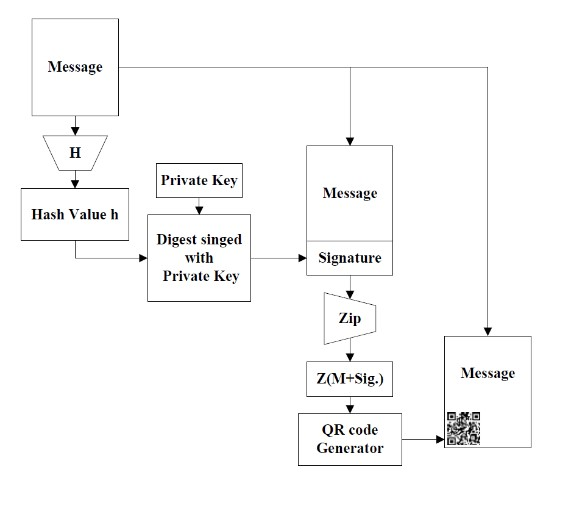
\includegraphics[width=\textwidth]{imgs/figure_2.1.1.jpg}
        \caption{Sender Process of Paper-based Document Authentication using Digital Signature and QR Code }
        \label{fig:Receiver Process of Paper-based Document Authentication using Digital Signature and QR Code}
        \end{figure}

\noindent{
    For this process, the message and the corresponding verification code in a form of QR code are printed on paper. After the message is composed, its hash value is generated. Then, the hash value h is encrypted with the private key of a sender resulting in the digital signature on the message M. After that, the message M and the digital signature are combined and compressed to reduce size so that they can be stored in a QR code. The compressed message and signature are fed into a QR code generator. After the QR code has been created, message M together with the QR code are printed on to paper and sent to a receiver. The simplified
process of sender is shown in Figure 2.1.1 \\
}
Receiver process
\begin{figure}[H]
    \centering
    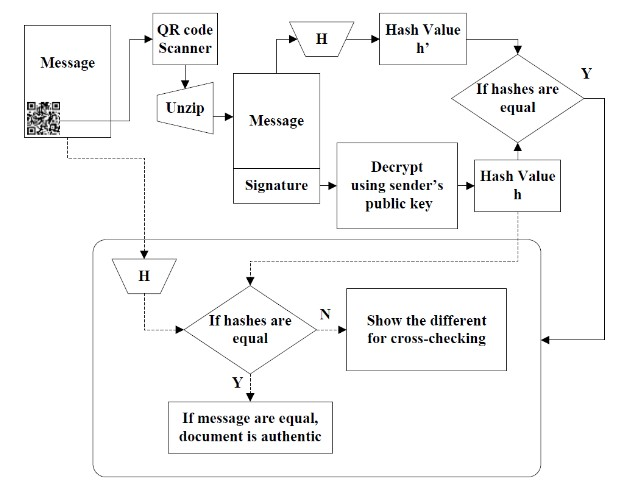
\includegraphics[width=\textwidth]{imgs/figure_2.1.2.jpg}
    \caption{Receiver Process of Paper-based Document Authentication using Digital Signature and QR Code }
    \label{fig:Receiver Process of Paper-based Document Authentication using Digital Signature and QR Code}
    \end{figure}
\noindent{
    When a receiver obtains the document from a sender, he/she may verify the authenticity of the document by scanning the document and processing the image as illustrated in Figure 2 (b). The verification process starts with checking the integrity of the information stored in the QR code. The information in the QR code consists of the message and the signature of the sender on the message, which are compressed. After scanning the QR code and uncompressing the data, the signature can be verified by comparing the hash value of the obtained message and the value from decrypting the signature using the sender’s public key. If both values are identical, the signature is valid. To validate the printed message, the Optical Character Recognition (OCR) must be employed. The hash value of the message obtained from the OCR is computed and compared with the hash value obtained from the message in the QR code. If they are identical, the printed message is authentic. However, if they are different, it cannot be concluded that the printed message has been modified. Further human review must be conducted. This is because the OCR may not be 100\% accurate. The message obtained from the QR code can be shown next to the printed message which can be visually inspected. \\
}
\vspace{1cm}



\noindent{\underline{CONCLUSION:}
Authenticity of paper-based documents can be achieved by using digital signatures and QR codes without accessing the database. The verification process can be done automatically if the OCR is accurate. Otherwise, human inspection is required. Even with this semi-automatic process, this proposed method facilitates the verification process. The inspector can see the differences between the printed message and the message in the QR code.\\
}

\section*{Towards a framework of A Secure E-Qualification Certificate System}



\textit{~ Lisha Chen-Wilson, Dr David Argles
School of Electronic and Computer Science
University of Southampton, United Kingdom
Published: 2010 Second International Conference on Computer Modeling and Simulation
}\\

\noindent{The paper-based certificates also  come with management problems. They are easily lost or  damaged, and they are hard to prove genuine when Presented. The field of e-Learning provides technological developments, such as e-portfolios, which are being explored as an improvement over paper-based portfolios in the job and course application process. However, forged certificates exist due to poor security in e-portfolio systems. Therefore, the students’ claimed achievements within e-portfolios need to be verified.\\

In order to solve the above problems, it is necessary to implement an electronic version of qualification certificates (e-certificate) that are at least as valid as the paper-based certificates, and can be used either as a standalone application or fitted within other applications, such as eportfolios. It needs to be easy to use and suit all levels of students while including high security methods to prevent forgery. The students need to have control over the usage of such e-certificate, and there must also be a verification method provided. We need to secure the e-certificate system, not just the e-certificate.\\
}

\begin{figure}[H]
    \centering
    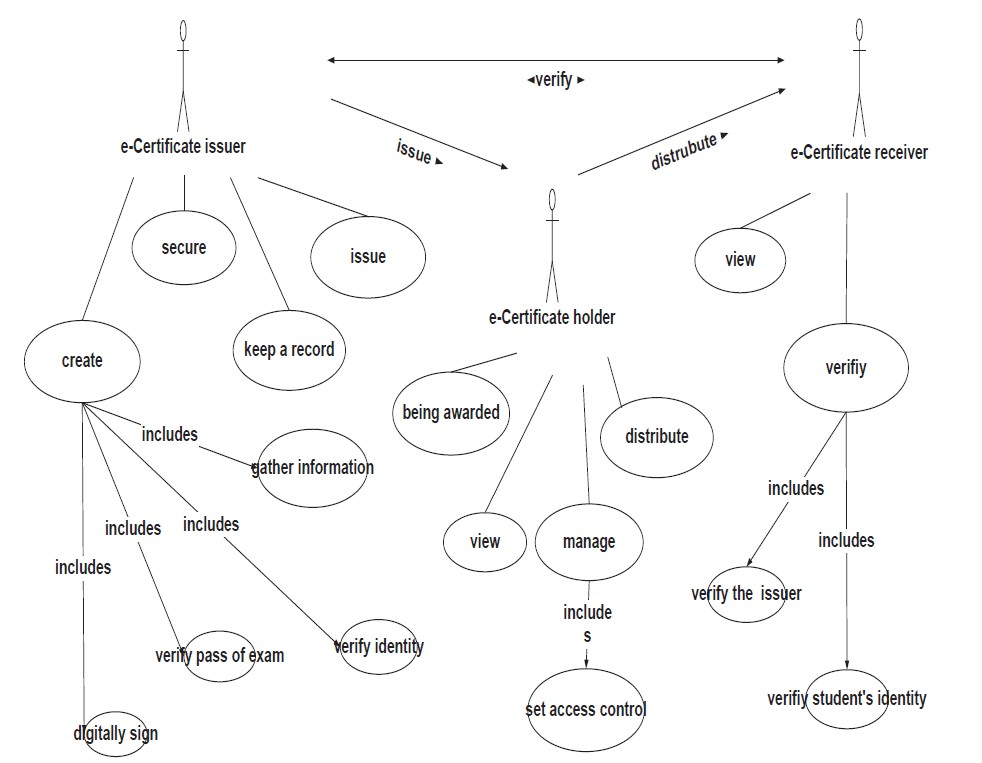
\includegraphics[width=\textwidth]{imgs/figure_2.2.1.jpg}
    \caption{Management of secure E-Qualification Certificate System
    }
    \label{fig:Management of secure E-Qualification Certificate System}
    \end{figure}

\noindent{An e-certificate issuer is a body that creates and issues the certificate, such as a college or a university. They may:}

\begin{itemize}
    \item Issue a huge range and amount of certificates

    \item Restrict database access control for any in coming verification request to minimize database attacks
  \end{itemize}

  \noindent{An e-certificate owner is the certificate holder who has successfully passed the qualification certification process and gained the award, such as a student or a graduate.
  An e-certificate reviewer is a body or a person who receives the certificate in support of an application. This may be an academic institution or an employer. They:
    }
    \begin{itemize}
        \item could be an individual or big organizations
        \item may receive e-qualification certificates as part of applications or within e-portfolios
\item may have few IT skills or may have a team of IT literate staff with high tech IT equipments
\item may need to check a few qualifications occasionally or may need to check a huge amount of qualifications efficiently
      \end{itemize}
    
\section*{Bitcoin: A Peer-to-Peer Electronic Cash System
}

\textit{by Satoshi Nakamoto }\\

\noindent{
    In this paper the author introduces a  purely peer-to-peer version of electronic cash that would allow online payments to be sent directly from one party to another without going through a financial institution. Digital signatures provide part of the solution, but the main benefits are lost if a trusted third party is still required to prevent double-spending.We propose a solution to the double-spending problem using a peer-to-peer network. The network timestamps transactions by hashing them into an ongoing chain of hash-based proof-of-work, forming a record that cannot be changed without redoing the proof-of-work. The longest chain not only serves as proof of the sequence of events witnessed, but proof that it came from the largest pool of CPU power. As long as a majority of CPU power is controlled by nodes that are not cooperating to attack the network, they'll generate the longest chain and outpace attackers. The network itself requires minimal structure. Messages are broadcast on a best effort basis, and nodes can leave and rejoin the network at will, accepting the longest proof-of-work chain as proof of what happened while they were gone.\\

\underline{Proof of work:}
To implement a distributed timestamp server on a peer-to-peer basis, we will need to use a proof of- work system similar to Adam Back's Hashcash, rather than newspaper or Usenet posts.The proof-of-work involves scanning for a value that when hashed, such as with SHA-256, the hash begins with a number of zero bits. The average work required is exponential in the number of zero bits required and can be verified by executing a single hash.For our timestamp network, we implement the proof-of-work by incrementing a nonce in the block until a value is found that gives the block's hash the required zero bits. Once the CPU effort has been expended to make it satisfy the proof-of-work, the block cannot be changed without redoing the work. As later blocks are chained after it, the work to change the block would include redoing all the blocks after it.\\
}

\begin{figure}[H]
    \centering
    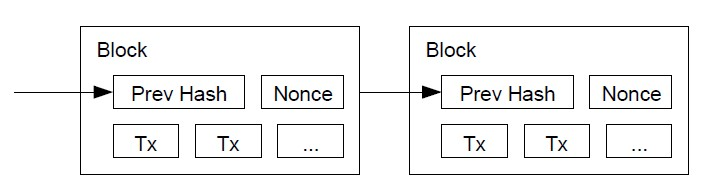
\includegraphics[width=\textwidth]{imgs/figure_2.3.1.jpg}
    \caption{Block representation of Blockchain
    }
    \label{fig:Block representation of Blockchain}
    \end{figure}

\noindent{
    The proof-of-work also solves the problem of determining representation in majority decision making. If the majority were based on one-IP-address-one-vote, it could be subverted by anyone able to allocate many IPs. Proof-of-work is essentially one-CPU-one-vote. The majority decision is represented by the longest chain, which has the greatest proof-of-work effort invested in it. If a majority of CPU power is controlled by honest nodes, the honest chain will grow the fastest and outpace any competing chains. To modify a past block, an attacker would have to redo the proof-of-work of the block and all blocks after it and then catch up with and surpass the work of the honest nodes. We will show later that the probability of a slower attacker catching up diminishes exponentially as subsequent blocks are added.\\
To compensate for increasing hardware speed and varying interest in running nodes over time, the proof-of-work difficulty is determined by a moving average targeting an average number of blocks per hour. If they're generated too fast, the difficulty increases.
}

\section*{ Educational Certificate Verification System Using Blockchain}

\textit{by  Dinesh Kumar K  Senthil P , Manoj Kumar D.S Publish:INTERNATIONAL JOURNAL OF SCIENTIFIC \& TECHNOLOGY RESEARCH VOLUME 9,ISSUE 03, MARCH 2020}\\

\noindent{
    The students' achievements available in the form of degree certificate, mark sheet, value added certificate, etc., will become an important weightage for recruitment or higher studies. The Education institution awards and degree certificates may have only the names of the institution and the student’s data. In this scenario there is a lack of effective anti forge mechanism, due to this many times the graduation certificate to be forged often is found. To solve the problem of fake certificates, the blockchain technology would store the certificate in digital form. The immutability nature of blockchain makes digital certificates in the distributed ledger very difficult to tamper or modify. Also, it is very easy to verify the originality of a digital certificate.
}

\begin{figure}[H]
    \centering
    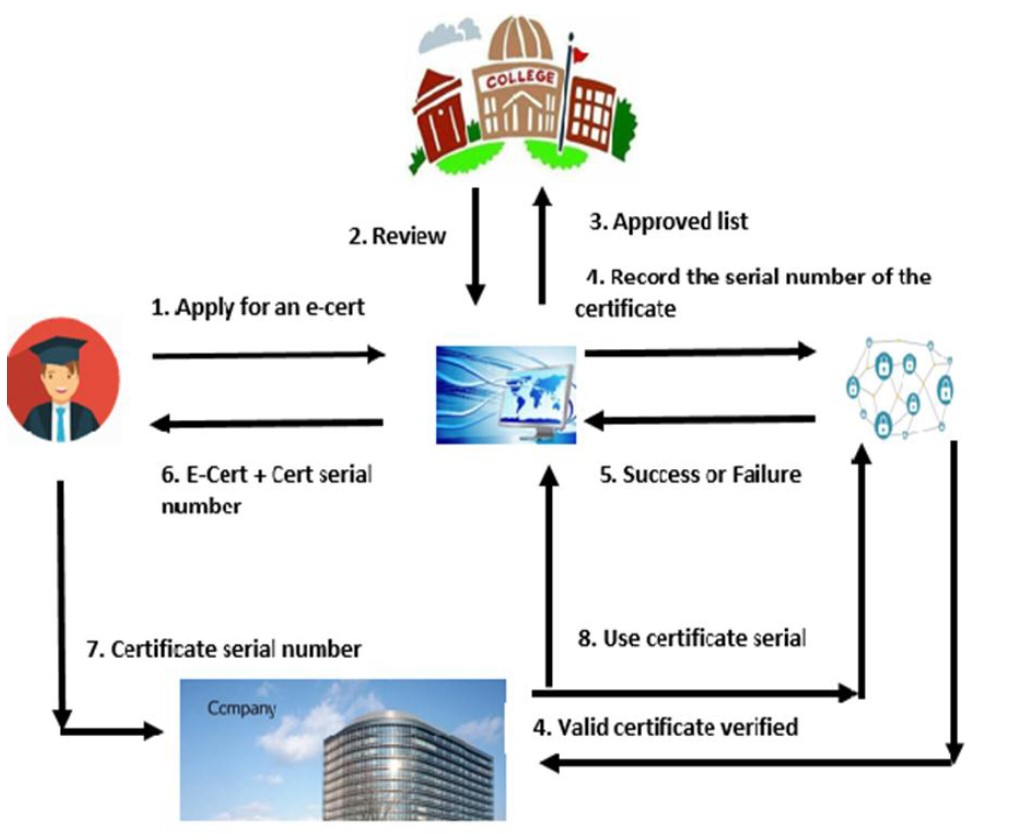
\includegraphics[width=\textwidth]{imgs/figure_2.4.1.jpg}
    \caption{Process of issuing digital certificates
    }
    \label{fig:Process of issuing digital certificates}
    \end{figure}

    \noindent{
The process of issuing digital certificates in the system is as follows. First step, generate the hash value for the certificate using double SHA256. Store the fixed length hash value as a transaction in the block. This transaction is validated by the members in the blockchain, once it is trusted as a valid transaction then the block is added with existing blockchain. Accepting and rejecting will be done using consensus algorithms . The consensus algorithm may be chosen based on number of nodes, and transactions. The system will generate the related QR code and inquiry string code to affix in the hardcopy certificate. The system provides the unit to authenticate the hardcopy certificate through phone scanner or website. The immutability nature of the distributed ledger, the system provides not only verification of certificate and also it stores the certificate in digital form forever\\}

\noindent{\underline{Result:}
Transparency and data immutability are the main features of blockchain application. It is a distributed ledger where nodes in the network validate and make final consensus to add the data in the network. The process of academic certificate generation is open and distributed among the parties where any organization or parties can verify information of any academic certificate using this blockchain system. The Ethereum blockchain also ensures data stored on the blockchain network is encrypted, therefore only the certificate owner can see and share this data as they wish. In conclusion, academic institutions are able to collaborate with other employers and publish credentials on the blockchain to eradicate fake educational certificates}


\section*{IPFS - Content Addressed, Versioned, P2P File System
}

\textit{by Juan Benet}\\

\noindent{
    The InterPlanetary File System (IPFS) is a peer-to-peer distributed le system that seeks to connect all comput- ing devices with the same system of les. In some ways, IPFS is similar to the Web, but IPFS could be seen as a single BitTorrent swarm, exchanging objects within one Git repository. In other words, IPFS provides a high throughput content-addressed block storage model, with content- addressed hyperlinks. This forms a generalized Merkle DAG, a data structure upon which one can build versioned systems, blockchains, and even a Permanent Web. IPFS combines a distributed hash table, an incentivized block ex-change, and a self-certifying namespace. IPFS has no single point of failure, and nodes do not need to trust each other.\\

IPFS is peer-to-peer; no nodes are privileged. IPFS nodes store IPFS objects in local storage. Nodes connect to each other and transfer objects. These objects represent les and other data structures. The IPFS Protocol is divided into a stack of sub-protocols responsible for different functionality:}

\begin{enumerate}
    \item  Identities - manage node identity generation and verification.
    \item Network - manages connections to other peers, uses various underlying network protocols. Configurable.
    \item Routing - maintains information to locate specific peers and objects. Responds to both local and remote queries. Defaults to a DHT, but is swappable.
    \item  Exchange - a novel block exchange protocol (BitSwap) that governs decent block distribution. Modeled as a market, weakly incentivizes data replication. Trade Strategies swappable
\item Objects - a Merkle DAG of content-addressed immutable objects with links. Used to represent arbitrary data structures, e.g. le hierarchies and communication systems.
\item Files - versioned le system hierarchy inspired by Git.
\item Naming - A self-certifying mutable name system.
\end{enumerate}


\section*{IPFS Based Storage Model for Blockchain}

\textit{by  Qinhong Zeng, Yi Li, Ping Chen, Xinghua Dong
2018 IEEE/WIC/ACM International Conference on Web Intelligence}\\

\noindent{
    This paper suggests making use of IPFS to store the certificates on IPFS.
    Take all the transactions of a block put it in a document and upload it on IPFS
    Further take the IPFS link as the transaction to the blockchain.
    This reduces the storage in blocks of blockchain there by reducing the load.
    }
    \begin{figure}[H]
        \centering
        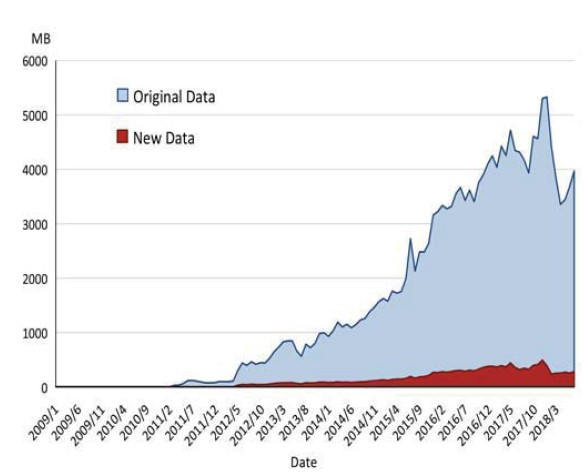
\includegraphics[width=\textwidth]{imgs/figure_2.6.1.jpg}
        \caption{Comparision of the sum of the block data in each before and after data processing
        }
        \label{fig:Comparision of the sum of the block data in each before and after data processing}
        \end{figure}
    \noindent{
       \underline{Results:}
It can be seen from the result that it has a certain degree of improvement in storage space,  security and new node synchronization speed.
}

\section*{Tamper-Proof Certificate Management System}

\textit{by Raghav, Nitish Andola, Rakhi Verma, S. Venketesan, Shekar Verma
2019 IEEE Conference on Information and Communication Technology
}\\

\noindent{
    Certificates are a proof of achievement/membership like University degrees and school certificates etc. Certificates as proof are essential in society but our current certificate management system is mostly analog, inefficient and amenable to forgery . Due to the ineffective anti-forge mechanism, forged certificates are becoming prevalent. To solve this problem, secure certificate management is proposed, then also security problems like privacy, transparency and forgeries still exist. We propose a tamper-proof certificate management using hyperledger which provides a secure anti-forge mechanism. Hyperledger has unmodifiable and other suitable properties of the blockchain that helps to minimize the problem of forgery. We use IPFS (Inter Planetary File System) for storing the certificate. The procedure for issuing the certificates is to first generate the degree of a student using a portal, meanwhile then calculate its hash value and encrypt it using asymmetric encryption. Then store file into
IPFS. Finally, we make a transaction that contains metadata of certificate which stores in the blockchain system. Then, chaincode is used for verification of the user's document. We also reduce the time complexity of searching and verifying the multiple documents of the same user. Our proposed work enhances the credibility of paper-based certificates, and also reduces the risk of forging certificates. We also show the performance of generating transactions in hyperledger.	}
    \begin{figure}[H]
        \centering
        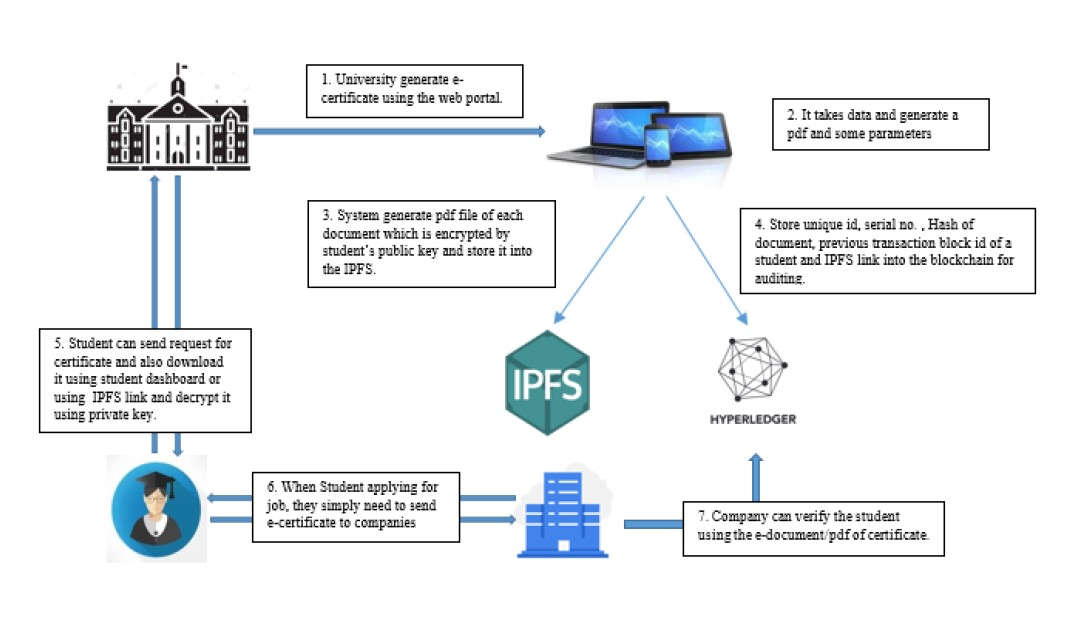
\includegraphics[width=\textwidth]{imgs/figure_2.7.1.jpg}
        \caption{Generating certificates using IPFS and hyperledger}
        \label{fig:Generating certificates using IPFS and hyperledger}
        \end{figure}
    \noindent{
       \underline{Results:}
       Our propose system provides integrity, privacy, transparency of certificate and anonymity of user
}

\section*{Blockchain-Blockcerts based Birth/Death Certificate Registration and Validation}

\textit{by Nitesh Sharma , Mohammad Afza, Asst. Prof Ankita Dixit
Department of Computer Science and Engineering, ABES Institute of Technology - Ghaziabad.
International Journal of Information Technology (IJIT) – Volume 7 Issue 5, Sep - Oct 2021}\\

\noindent{
    As we know that Birth/Death Certificates are very essential documents. Birth Certificate can be used as proof of an individual’s age, for academics, for jobs and can be used as an identity for various government documents (Passport, Driving License, Voter-ID, etc.). Likewise, Death Certificates can be used by the family of deceased to inherit property, to claim insurance benefits and used by the government to maintain population statistics. In the current scenario, due to the complex procedure of applying and getting a certificate, nearly half of the world’s population does not have a birth certificate. Also, authentication of a valid certificate is a laborious task. At the same time, due to the presence of hard copy, missing certificates become a crucial problem and re-issuing of that certificate is a hectic process. Presently, the digital certificate is a way to tackle the problem of missing certificates still it is not sufficient as it can tamper easily.\\

Therefore, the objective of this paper is to give the solution to issue Birth/Death certificates and validation of certificates using Blockcerts which is based on Blockchain Technology. Blockcerts is used for issuing and verifying a blockchain-based formal transaction. Blockchain is a shared distributed, decentralized database system used to store information and this information cannot tamper easily. It also provides security services like confidentiality, authentication, integrity and access control list of data
	}
    \begin{figure}[H]
        \centering
        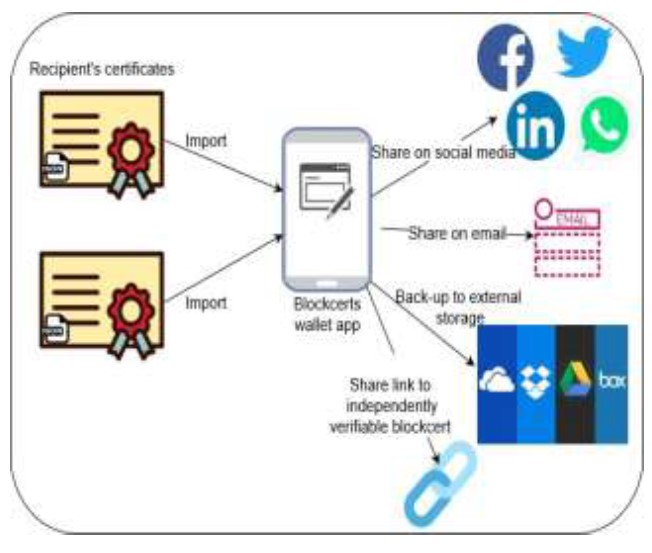
\includegraphics[width=\textwidth]{imgs/figure_2.8.1.jpg}
        \caption{Solution that will replace the conventional approach of birth/death certificate generation}
        \label{fig:Solution that will replace the conventional approach of birth/death certificate generation}
        \end{figure}
    \noindent{
       \underline{Results:}
       Our propose system provides integrity, privacy, transparency of certificate and anonymity of userIn this paper, we presented a solution that will replace the conventional approach of birth/death certificate generation. We have used blockchain technology and Blockcerts in the process of birth/death certification and validation. The solution includes registration of birth/death, creation of JSON file (digital certificate), public-private key cryptography to Achieve confidentiality using encryption and digital signature.


}

\chapter{PREREQUISITES}

\section{Merkle Trees}
\noindent{
Merkle trees are created by repetitively hashing pairs of nodes until only one hash is left, this hash is better called the Merkle Root or the Root Hash. They are constructed from the bottom, from the hashes of individual transactions called Transaction IDs. Thus every leaf node is a hash of transactional data, and each non-leaf node is a hash of its previous hash. }
\begin{figure}[H]
    \centering
    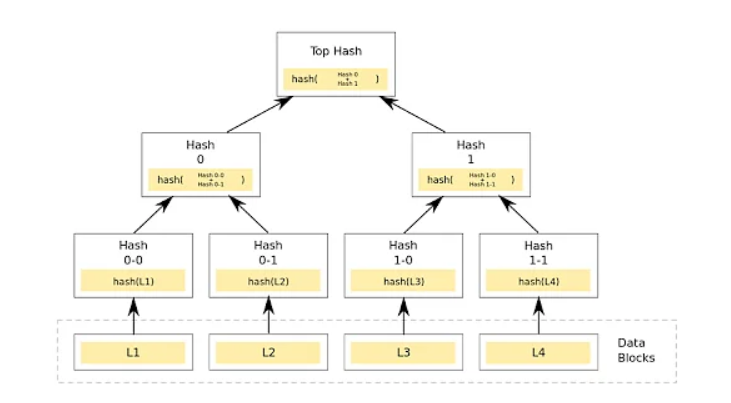
\includegraphics[width=\textwidth]{imgs/merkel_tree.png}
    \caption{Working of Merkle Tree}
    \label{fig:Working of Merkle Tree}
    \end{figure}
    \section{SHA-256}
    \noindent{ 
    SHA 256 is a math process that generates a 256 bit (64 character long) random sequence of letters and numbers (hash) out of any input.Hashing is used to make storing and finding information quicker because hashes are usually shorter and easier to find. The number of possible combinations of letters and numbers produced by SHA 256 exceeds the number grains of sand on Earth! That makes guessing the data hidden within the hash virtually impossible. Hashes cannot be reversed.}    

    \section{Proof Of Work ( POW )}
\noindent{The proof-of-work protocol, Ethash, requires miners to go through an intense race of trial and error to find the nonce for a block. Only blocks with a valid nonce can be added to the chain.\\
When racing to create a block, a miner will repeatedly put a dataset, that you can only get from downloading and running the full chain (as a miner does), through a mathematical function. The dataset gets used to generate a mixHash below a target nonce, as dictated by the block difficulty. The best way to do this is through trial and error.\\
Once generated, this is incredibly easy for other miners and clients to verify. Even if one transaction were to change, the hash would be completely different, signaling fraud.
Hashing makes fraud easy to spot. But proof-of-work as a process is also a big deterrent to attacking the chain\\
The objective of proof-of-work is to extend the chain. The longest chain is most believable as the valid one because it's had the most computational work done. Within Ethereum's PoW system, it's nearly impossible to create new blocks that erase transactions, create fake ones, or maintain a second chain. That's because a malicious miner would need to always solve the block nonce faster than everyone else.}


\section{Proof Of Stake ( POS )}
\noindent{Proof of stake is a type of consensus mechanism used by blockchain networks to achieve distributed consensus.It requires users to stake their ETH to become a validator in the network. Validators are responsible for the same thing as miners in proof-of-work: ordering transactions and creating new blocks so that all nodes can agree on the state of the network.
Proof-of-stake comes with a number of improvements to the proof-of-work system:
better energy efficiency – you don't need to use lots of energy mining blocks
lower barriers to entry, reduced hardware requirements – you don't need elite hardware to stand a chance of creating new blocks
stronger immunity to centralization – proof-of-stake should lead to more nodes in the network
stronger support for shard chains – a key upgrade in scaling the Ethereum network.}
 
\section{Digital signature }
\noindent{It uses public key cryptography to validate and ensure  authenticity and integrity of the signed information. Let’s have a look at how digital signature uses public key cryptography for signing and verification operations.}
\begin{itemize}
\item Authentication: When a verifier validates a digital signature using the sender's public key, he is confident that the signature is of the sender with an associated secret private key.
\item Data Integrity: If an attacker edits the data, the digital signature verification at the receiver end fails. The hash of updated data and the verification algorithm’s result will not match. As a result, the receiver can securely reject the message.
\item Non-repudiation: Because the signature key is known only to the signer, he can create a unique signature on a given data. In the event of a future disagreement, the receiver might offer the data and digital signature to a third party as evidence.
\end{itemize}\


\section{51\% Attack}
\noindent{A 51\% attack refers to an attack on a blockchain by a group of miners controlling more than 50\% of the network's mining hash rate or computing power. The attackers would be able to prevent new transactions from gaining confirmations, allowing them to halt payments between some or all users.}

\section{Blockchain}
\textit{Decentralized.Transparent. Anonymous. Consensus Base. Immutable. Open Source.\\}
\underline{Blockchain Structure}\\

Each block in the blockchain contains five elements which are: 
\begin{itemize}
\item \textbf{Main Data}. The data depends on the type of transaction; it is generally a transfer between nodes A and B however it can be of any type like money transfer or record transfer.
\item \textbf{Hash of the Previous Block}. When a transaction is executed, its hash is generated and broadcasted to the network. There are several hashing algorithms in use but the most dominant is the Merkle Tree. This algorithm allows easy hash and easy de-hash options which is why Merkle Trees are a common choice.
\item \textbf{Hash of the Current Block}. The final hash value is recorded in the block header (hash of current block), while the content itself is stored in the body of the block. Blocks are generally bound to a size hence allowing a limited number of transactions per block.
\item \textbf{Timestamp}. The time the block was generated.
\item \textbf{Nonce and Other Information}. Like the signature of the block, Nonce value, or other data that the user defines.
\end{itemize}
\begin{figure}[H]
    \centering
    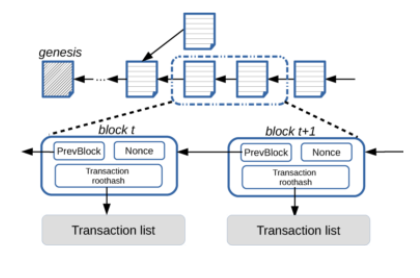
\includegraphics[width=\textwidth]{imgs/blockchain_block_structure.png}
    \caption{Detail view of a block of blockchain}
    \label{fig:Detail view of a block of blockchain}
    \end{figure}

\vspace{1cm}

\textit{SECURITY THEMES FOR CERTIFICATES IN BLOCKCHAIN\\}
Certificates on a blockchain must fulfill certain essential themes namely,
\begin{itemize}
    \item Authentication: identifying whether the user is authentic i.e. the user is registered on the server or the platform
    \item Authorization:process of giving access to specific resources only to authenticated users.
    \item Confidentiality: it's about maintaining secrecy of information between the user and the platform/server.
    \item Ownership: it specifies who owns the data or some resource.
    \item Privacy: it's about maintaining confidentiality about the user details
\end{itemize}

\vspace{1cm}

\textit{LIMITATIONS OF TRADITIONAL VERIFICATION\\}
This section discusses the limitations of the traditional verification system. Existing verification methods do not guarantee records that are not sealed, secured, tamper-proof, and authenticated. five limitations of traditional verification systems which are ownership, availability, dependency on third-party agencies, time consumption and cost. \\
Explanation of each limitation as follows:
\begin{itemize}
    \item Ownership:
The certificate ownership does not automatically appear to the individuals.
\item Availability:
Physical documents may be lost or damaged. Hence, individuals who lose them cannot readily obtain duplicates.
\item Dependency: on third-party agencies
Many organizations depend on third-party verification agencies to contact issuing authorities and verify document authenticity.
\item Time utilization:
The process is time-consuming. The speed of verification depends on the response time of issuing authorities and their location.
\item Cost:
A fee is charged for each verification for the certificate or document.
\end{itemize}


\begin{table}[H]
    \normalsize
    \begin{center}
    \begin{tabular}{|m{4cm}| m{5.5cm}|m{5.5cm}|}
        \hline
        \textbf{PARAMETERS} & \textbf{BLOCKCHAIN} & \textbf{TRADITIONAL VERIFICATION SYSTEM}\\
        \hline
    DOCUMENT PERSPECTIVE & It can avoid the risk of losing or falsifying paper documents. & In this traditional system all the contents are in paper formats.\\
    \hline
    COST-EFFECTIVE & Blockchain helps in transferring the right to control and store the applicant’s personal data to the applicant himself. & Institutions can reliably and responsibly store documents and offer access to the applicants at the request of employers and authorities.\\
    \hline
    PAYMENT METHODS & No payments for intermediate services. & There is a payment for each and every third-party service.\\
    \hline
    DURING TRANSACTION & Transparency of transactions increased. & Transparency of transactions is less.\\
        \hline

        SECURITY & More secure, records are stored in blocks. & Less secure because records are stored in a local database.\\

        \hline

        IMMUTABILITY &
Records to be written and stored permanently, without the possibility of modifications. &
Records are in paper format, so the chance of modifying certificates gets increased.\\

\hline
EFFICIENCY &
More efficient. &
Less efficient. \\

\hline
    \end{tabular}  
    \caption{Comparision of traditional systems and blockchain}
    \label{table-example}
    \end{center}
    \end{table}

\section{IPFS}
\noindent{ IPFS (Inter Planetary File System) is a peer- to peer hypermedia protocol and distributed file system. It has a block storage model with hyperlinks to address the contents forming a Merkle Directed Acyclic Graph. Since IPFS is distributed, it has no single point of failure. IPFS represents a file by the hash on it, instead of representing it by which server it is stored on.
Storing large amounts of data on Ethereum can be very expensive. Content-based addresses that IPFS returns are 46 bytes in size which is a tiny amount considering the size of files. It is cheaper to publish a file on IPFS and store their content-based address on the Ethereum blockchain. \\}

\vspace{1cm}
\textit{HOW IPFS WORKS? }

\begin{itemize}
    \item 
    When you add a file to IPFS, your file is split into smaller chunks, cryptographically hashed, and given a unique fingerprint called a content identifier (CID). This CID acts as a permanent record of your file as it exists at that point in time.
    \item When other nodes look up your file, they ask their peer nodes who's storing the content referenced by the file's CID. When they view or download your file, they cache a copy — and become another provider of your content until their cache is cleared.
    \item A node can pin content in order to keep (and provide) it forever, or discard content it hasn't used in a while to save space. This means each node in the network stores only content it is interested in, plus some indexing information that helps figure out which node is storing what.
    \item If you add a new version of your file to IPFS, its cryptographic hash is different, and so it gets a new CID. This means files stored on IPFS are resistant to tampering and censorship — any changes to a file don't overwrite the original, and common chunks across files can be reused in order to minimize storage costs.
    \item However, this doesn't mean you need to remember a long string of CIDs — IPFS can find the latest version of your file using the IPNS decentralized naming system, and DNSLink can be used to map CIDs to human-readable DNS names.
\end{itemize}

\vspace{1cm}
\textit{Advantages of IPFS}

\begin{itemize}
   \item \underline{Archivists}
Storing archival data using IPFS enables deduplication, clustered persistence, and high performance — empowering you to store the world's information for future generations.

\item \underline{Service providers}
Providing large amounts of data to users? Storing on IPFS could help you slash bandwidth costs thanks to its use of secure, peer-to-peer content delivery.

\item \underline{Researchers}
If you're working with or distributing large datasets, storing that data using IPFS can help speed up performance and unlock decentralized archiving.

\item \underline{Blockchain developers}
IPFS content addressing enables you to store large files off-chain and put immutable, permanent links in transactions — timestamping and securing content without having to put the data itself on-chain.

\item \underline{Content creators}
IPFS empowers creators to build and share on the decentralized web — whether that's delivering content free from intermediary control or minting NFTs that stand the test of time.

\item \underline{Offline users}
High-latency networks cause major obstacles for those with poor internet infrastructure. Peer-to-peer IPFS offers resilient access to data independent of latency or backbone connectivity.

\end{itemize}

\begin{table}[H]
    \normalsize
    \begin{center}
    \begin{tabular}{|m{7cm}| m{7cm}|}
        \hline
        \textbf{HTTP} & \textbf{IPFS} \\
        \hline
        It uses a centralized client server approach &
It uses a decentralized peer to peer approach.\\
        \hline
        Data is requested using the address on which data is hosted &
Data is requested using the cryptographic hash of that data \\
        \hline
        Data cannot be accessed if the server is down or fails or any link gets broken & 
Data is copied to multiple nodes, hence it can be accessed whenever needed.\\
        \hline
        The bandwidth provided is low, as multiple clients request from a single server at the same time. &
        Bandwidth is high, as data is requested from the closest peer who has the copy of that data.\\
        \hline
        One has to set up a hosting server or pay for one, in order to make content publicly available. &
Uploading content on the IPFS network does not require a host server, every node hosts the data on the network.\\
        \hline
        HTTP is well established as an industry standard, this is where HTTP has an upper hand. &
IPFS is relatively newer and is not yet as popular as HTTP.\\
\hline 
HTTP support is inbuilt on almost all machines. &
To run IPFS you need to access it using the HTTP to IPFS portal or manually set up an IPFS node on your machine.\\

\hline
HTTP is used by almost everyone to access the web.	&
Currently, there is a shortage of IPFS nodes due to its low popularity among the laymen.\\
\hline
    \end{tabular}  
    \caption{HTTP v/s IPFS}
    \label{table-example}
    \end{center}
    \end{table}

\section{Ethereum}
\noindent{
    Ethereum is a technology that lets you send cryptocurrency to anyone for a small fee. It also powers applications that everyone can use and no one can take down.\\
It's the world's programmable blockchain.
Ethereum builds on Bitcoin's innovation, with some big differences.\\
Both let you use digital money without payment providers or banks. But Ethereum is programmable, so you can also use it for lots of different digital assets – even Bitcoin!
This also means Ethereum is for more than payments. It's a marketplace of financial services, games and apps that can't steal your data or censor you.}

\section{Smart Contract}
\noindent{A smart contract is a self-executing contract with the terms of the agreement between buyer and seller being directly written into lines of code. The code and the agreements contained therein exist across a distributed, decentralized blockchain network.Smart contracts render transactions traceable, transparent, and irreversible.}

\end{document}
